\documentclass[runningheads]{llncs}
\usepackage{graphicx}
\usepackage{amsmath,amssymb}
\usepackage{ruler}
\usepackage{color}
\usepackage[width=122mm,left=12mm,paperwidth=146mm,height=193mm,top=12mm,paperheight=217mm]{geometry}
\begin{document}
\pagestyle{headings}
\mainmatter

%
\def\ECCV16SubNumber{16}
\def\GroupNumber{16}
\title{Evaluation of Spectral Normalization for GANs Using Inception Score}
\titlerunning{Evaluation of Spectral Normalization for GAN using Inception Score}
\authorrunning{Authors}
\author{Eysteinn \textsc{Gunnlaugsson},
	Egill \textsc{Vignisson},
	Charles \textsc{Hamesse}}
\institute{Group \GroupNumber}
\maketitle

%
\begin{abstract}
The abstract should summarize the contents of the paper. LNCS guidelines
indicate it should be at least 70 and at most 150 words. It should be set in 9-point
font size and should be inset 1.0~cm from the right and left margins. \dots
\keywords{Generative adversarial networks, generative models, image generation}
\end{abstract}

%
\section{Introduction}
Motivate the problem you are trying to solve, attempt to make an intuitive description of the problem and also formally define the problem. (1-2 pages including title, authors and abstract)


In this project, we will implement a number of different Generative Adversarial Networks (GANs) \cite{goodfellow2014generative} for image generation.
 
 
We plan to at least implement DCGAN \cite{DBLP:journals/corr/RadfordMC15} with the new Spectral Normalization \cite{miyato2018spectral}. On top of that and if time allows, we will also implement different losses such as LSGAN \cite{mao2017least} or WGAN \cite{arjovsky2017wasserstein}, and various training improvement techniques such as mini-batch discrimination \cite{salimans2016improved}. 

For evaluating the performance of these GANs, we will implement the inception score metric as described in \cite{salimans2016improved}. We already have made up a dataset of 30K animal pictures (mostly reptiles), fetched from the Flickr API. If that turns out to be too few or not suitable for any reason we will fall back to using CIFAR-100 or ImageNet (or a subset of these).  


\section{Background}
We present the framework of GANs starting with the original paper by Ian Goodfellow \cite{goodfellow2014generative} then describe more recent advances in a chronological order, as depicted in Figure \ref{fig:background-timeline}. 
% Summarize a few notable approaches/papers tackling the same problem. The selection should cover different possible techniques that can be (have been) used for the same task with success. Also, it is good to mention other recognition/synthesis tasks that use the same deep learning technique as yours. (1-2 pages)

\begin{figure}
\centering
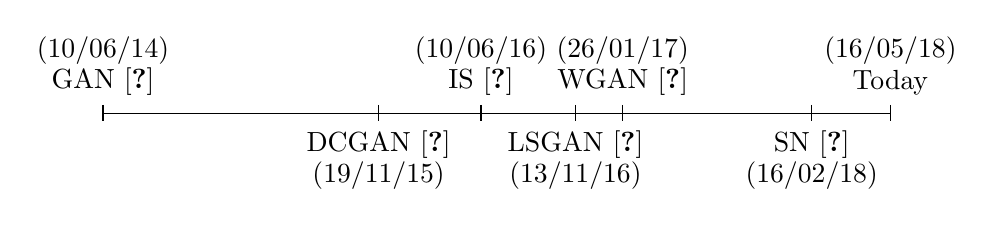
\begin{tikzpicture}
\draw (0,0) -- (10,0);

% draw vertical lines
\foreach \x in {0,3.5,4.8,6.0,6.6,9.0,10.0}
\draw (\x cm,3pt) -- (\x cm,-3pt);

% draw nodes
% 1 yr is roughly 2.5 units
\draw (0,0) node[above=3pt] {GAN \cite{goodfellow2014generative}};
\draw (0,0) node[above=14pt] {(10/06/14)};

\draw (3.5,0) node[below=3pt] {DCGAN \cite{DBLP:journals/corr/RadfordMC15}};
\draw (3.5,0) node[below=14pt] {(19/11/15)};

\draw (4.8,0) node[above=3pt] {IS \cite{salimans2016improved}};
\draw (4.8,0) node[above=14pt] {(10/06/16)};

\draw (6,0) node[below=3pt] {LSGAN \cite{mao2017least}};
\draw (6,0) node[below=14pt] {(13/11/16)};

\draw (6.6,0) node[above=3pt] {WGAN \cite{arjovsky2017wasserstein}};
\draw (6.6,0) node[above=14pt] {(26/01/17)};

\draw (9.0,0) node[below=3pt] {SN \cite{salimans2016improved}};
\draw (9.0,0) node[below=14pt] {(16/02/18)};

\draw (10.0,0) node[above=3pt] {Today};
\draw (10.0,0) node[above=14pt] {(16/05/18)};

\end{tikzpicture}
\caption{Major contributions in the field of Generative Adversarial Networks.}
\label{fig:background-timeline}
\end{figure}


% 2014 jun 10: GAN
% 2015 nov 19: DCGAN
% 2016 jun 10: IS
% 2016 nov 13: LSGAN
% 2017 jan 26: WGAN 
% 2018 feb 16: SN  
% 2018 may 16: Today 

In this work, we consider all of the techniques mentioned in Figure \ref{fig:background-timeline} except LSGAN \footnote{As we progressed in our work, we figured out it was more relevant to investigate further with WGAN-related techniques than implementing a broad spectrum of techniques without really going in-depth.}.

\subsection{Generative Adversarial Networks} 
Generative Adversarial Networks (GANs) were first introduced in \cite{goodfellow2014generative}. They are a class of generative models trained in a adversarial manner by opposing two networks: a generative network $G$ that learns the data distribution and a discriminative network $D$ that tries and estimates the probability that a given sample came from the real training data rather than a generation from $G$. 
 
The objective for $G$ is to maximize the probability of $D$ making a mistake, and the objective for $D$ is to minimize that same probability. This framework corresponds to a minimax two-player game. In the space of arbitrary functions $G$ and $D$, a unique equilibrium solution exists, with $G$ recovering the real data distribution and $D$ equal to 0.5 everywhere, meaning it's unable to distinguish the real images from the ones generated by $G$. Since $G$ and $D$ are (de-)convolutional networks, both can be trained using available backpropagation techniques.

To learn the distribution $p_g$ over the real data $\bm{x}$, $G$ starts from sampling input variables $\bm{z}$ from a distribution of our choice $p_z(\bm{z})$, then maps the input variables $\bm{z}$ to space $G(\bm{z}; \theta_g)$ that should, after training, resemble the training data space. The discriminator, $D$, maps images to a boolean $D(\bm{x}; \theta_d)$ indicating whether images are from training data or generated from $G$. The orignal minimax objective for GANs is defined as:
\begin{equation}
\label{eq_gan}
\min_G \max_D V_{\text{\tiny GAN}}(D, G) = \mathbb{E}_{\bm{x} \sim p_{\text{data}}(\bm{x})}[\log D(\bm{x})] + \mathbb{E}_{\bm{z} \sim p_{\bm{z}}(\bm{z})}[\log (1 - D(G(\bm{z})))] .
\end{equation}

\subsection{Deep Convolutional Generative Adversarial Networks}
Building upon Goodfellow's work \cite{goodfellow2014generative}, Radford et al. apply the GAN framework to computer vision, bridging the gap between the success of Convolutional Neural Networks (CNNs) for supervised learning and GANs for unsupervised learning \cite{DBLP:journals/corr/RadfordMC15}. Training on various image datasets, authors show that the adversarial pair learns a hierarchy of features in both the generator and discriminator. 

\subsection{Inception Score}
The Inception Score (IS) is first presented in \cite{salimans2016improved}. This work (originating from OpenAI, whose team includes author of the original GAN paper Ian Goodfellow) presents a variety of new architectural features and training procedures meant to improve the training of GANs. Amongst other things, authors make the observation that GANs lack an objective function, making it difficult to compare the performance of different models. In the context of image generation, an intuitive performance metric can be obtained by human annotators assessing the quality of the generated images. However, this method isn't as scalable as one would wish for obvious reasons. The inception score is proposed as an alternative, and is shown to correlate well with human evaluation. 

We describe the method briefly. By applying the Inception model \cite{inceptionv2} to all generated images, we get the conditional label distribution $p(y|\bm{x})$. Images that contain meaningful objects should have a conditional label distribution $p(y|\bm{x})$ with low entropy. Moreover, we expect the model to generate varied images, so the marginal $\int p(y|\bm{x} = G(z))dz$ should have high entropy. By combining these two requirements, the proposed metric becomes: 

%$\exp( \mathbb{E}_{\bm{x}} \text{KL} (p(y|\bm{x})||p(y)))$, where results are exponentiated so that values are easier to compare.
% In \cite{Barrat2018IS} the Inception score is defined  as:
\begin{equation}
\label{eq_IS}
\begin{split}
\text{IS}(G) = \exp \big(\mathbb{E}_{\bm{x} \sim p_{\text{data}}(\bm{x})}D_\text{KL}(p(y|\bm{x})||p(y))\big).
\end{split}
\end{equation}

Here $D_{KL}$ is known as the Kullback-Leibler divergence and it measures how one probability distribution diverges from another by using a logarithmic difference:
\begin{eqnarray}
	D_{\mathrm {KL} }(P\|Q)=\int _{-\infty }^{\infty }p(x)\,\log {\frac {p(x)}{q(x)}}\,dx,
\end{eqnarray}
where $p(y|\bm{x})$ is the conditional label distribution while $p(y)$ is the  marginalized label distribution, i.e. $p(y)=\int_{\bm{x}} (p(y|\bm{x})p_g(\bm{x}) d\bm{x}$. In order to calculate the score we replace $p(y)$ with the empirical marginal class distribution $\hat{p}(y) = \sum^N_{i=1} p(y|\bm{x}^i)$ and estimate the expectation using the basic Monte Carlo estimator yielding:

\begin{equation}
\label{eq_IS2}
\begin{split}
\text{IS}(G) = \exp\left(\sum^N_{i=1}D_{\mathrm{KL}}(p(y|\bm{x}^i)||\hat{p}(y))\right).
\end{split}
\end{equation}


\subsection{WGAN}
The Wasserstein GAN (WGAN) algorithm is proposed as a consequence to various  observations on how we usually measure the distance between the model distribution and the real distribution. In fact, the choice of divergence functions has a huge impact on how the discriminator will manage to classify samples as real or fake, and in turn how the generator will be led to adjust its parameters to mimic the real distribution. Authors show how the Earth Mover (EM) distance behaves in comparison to popular probability distances and divergences used in the context of learning distributions. WGANs are developed by making GANs minimize a reasonable and efficient approximation of the EM distance, working under the assumption that the discriminator functions are $K$-Lipschitz continuous. For a parameterized family of functions $\{ f_w \}_{w \in \mathcal{W}}$ that all have the $K$-Lipschitz continuity property, the discriminator objective is defined as:
\begin{equation} \label{eq:wgan}
\max_{w \in \mathcal{W}} \mathbb{E}_{x \sim p_{\text{data}}(x)}[f_w(x)] -
\mathbb{E}_{z \sim p(z)} [f_w(g_\theta (z)].
\end{equation}
As a result, one of the most compelling practical benefits of WGANs is the ability to continuously estimate the EM distance by training the discriminator to optimality. Various ways to ensure Lipschitz continuity are described, including gradient penalty or weight clipping. For the latter, however, author note that it is ``clearly terrible way to enforce a Lipschitz constraint'' \cite{arjovsky2017wasserstein}.
% Recommended clip limit is 0.01

\subsection{Spectral Normalization}
\label{sec:bg-sn}

Spectral normalization \cite{miyato2018spectral} was introduced in an effort to try and make the training of GANs more stable and the original paper received very positive criticism. \footnote{As a matter of fact, this has been posted on the \href{https://openreview.net/forum?id=B1QRgziT-}{peer-reviewing platform}:
\begin{quote}
\textit{``This is a great paper! I don't think this paper explains the importance of its results nearly enough and I'm concerned that it may not be obvious what a breakthrough it is just from skimming the abstract.''} - Ian Goodfellow
\end{quote}
}. As we noted in the previous section, Lipschitz continuity is a property of interest for GANs. More specifically, the assumption for the loss of Wasserstein GANs is that the functions yielded by the discriminator are $K$-Lipschitz continuous for some constant $K$. Spectral normalization aims to control the Lipschitz constant of this discriminator function $f$ by constraining the spectral norm of each layer 
$
g_l : \bm{h}_{l-1} \mapsto W^{l} \bm{h}_{l-1}
$. We briefly review the method, but the interested reader will find a more comprehensive explanation in the original paper. 

By definition, the Lipschitz norm $\|g\|_{\rm Lip}$ is equal to $\sup_{\bm{h}} \sigma (\nabla g(\bm{h}))$, with $\sigma (A)$ being the spectral norm of the matrix $A$ (which is equivalent to the largest singular value of $A$). Therefore, for a linear layer $g_l$, the norm is given by $\|g_l\|_{\rm Lip} = \sup_{\bm{h}} \sigma (\nabla g_l(\bm{h})) = \sup_{\bm{h}} \sigma (W_l) = \sigma (W_l) $. Now, if the Lipschitz norm of the activation function $\|a_l\|_{\rm Lip}$ is equal to 1 (a condition that ReLU or Leaky ReLU satisfy \todo{cite}), we can use the composition inequality $\|g_1\circ g_2\|_{\rm Lip}\leq\|g_1\|_{\rm Lip}\cdot\|g_2\|_{\rm Lip}$ and define the bound on $\|f\|_{\rm Lip}$:
%
% The last layer should not have an activation function in this context
% However we can omit (nobody will notice I guess) or add an indicator function as exponent
%
\begin{align}
 	\|f\|_{\rm Lip} \leq &  \prod_{l=1}^{L+1} \|a_{l}\|_{\rm Lip} \|g_{l}\|_{\rm Lip} = \prod_{l=1}^{L+1} \sigma (W^{l}). \label{eq:ineq_lip}
\end{align}
For each layer, spectral normalization alters the weight matrix $W_l$ so that it satisfies the Lipschitz constraint $\sigma (W_l) = 1$:
\begin{align}
\bar{W_l}_{\rm SN}(W_l) := W_l / \sigma (W_l) \label{eq:sn},
\end{align}
enforcing the upper bound of 1 for $\|f\|_{\rm Lip}$ using the inequation \ref{eq:ineq_lip}.


\section{Approach}

Describe the final approach you are take for this problem.
For instance, here you would describe the details of the network’s
architecture. What training parameters and techniques you have used.
The computational complexity of your model. And similar questions.
To help explain your approach please make figures to accompany your
text description. (1-3 pages)

%Not sure these sections actually belong here do with them as you please
\subsection{Data Collection}
%not sure if this is actually something we want to include and if so where it should be introduced so feel free to change it
%TODO possibly add a reference instead of the hyperlink
During experimentation we mostly relied on the popular benchmark dataset \href{https://www.cs.toronto.edu/~kriz/cifar.html}{CIFAR-10}, however an additional data set was collected using \href{https://www.flickr.com/services/api/}{Flickr's API}. Due to varying amounts of quality pictures of objects that would be interesting to base the image generation on, a collection that included mostly different reptiles with a fair amount of arachnid's thrown into the mix was ultimately settled upon therefore this data set will be referred to as the Reptiles form here on. In total the data set is made up of approximately 20k color images all re-sized to dimensions of 108x108x3 before training was conducted. Examples of images can be seen in figure \ref{fig:reptiles}.

\begin{figure}[H]
\centering
\includegraphics[width=\textwidth]{figures/reptiles.png}
\caption{Examples from the Reptiles data set}
\label{fig:reptiles}
\end{figure}






\section{Experiments} In this section, you should
present the results you achieved with various experiments. The results
can be presented in tables, plots, etc. 

The purpose of the project is to analyze the nature and effectiveness of different GAN architectures as well as different improvement options. The different models  but in order to do so a frame of reference was needed 

\subsection{DCGAN}
In order to establish a frame of reference a plain vanilla version of DCGAN using 

\subsection{DCGAN with Spectral Normalization}

\subsection{LSGAN}

\subsection{WGAN}

\section{Conclusions}
%Explain what conclusions you can draw from these set of experiments? The set of experiments and results reported here should justify some of the design choices described in the previous sections. (3-6 pages)
Figure  \ref{fig:exp-all-is} compares the Inception score for all tested network settings. Even though the Inception score of the basic DCGAN is not improved using the evaluated methods the overall quality of the generated images is clearly higher and the presence of mode collapse is significantly reduced or even non-existent for GAN's where spectral normalization, Wasserstein loss or both were added. In addition to these improvements both the D loss and G loss were much smoother during training. Having smoother losses allows for much better monitoring of the networks behavior during the training process leading to a much more intuitive hyper parameter tuning and debugging process. 
\begin{figure}[H]
\centering
\includegraphics[width=\textwidth]{../code/results/figures/all_cifar10_is.png}
\caption{All evaluated models - Inception score, training on CIFAR10}
\label{fig:exp-all-is}
\end{figure}



%\todo{to justify the use of WGAN / the need for loss smoothness: Plotting these learning curves is not only useful for debugging and hyperparameter searches, but also correlate remarkably well with the observed sample quality. (taken from WGAN paper) }

\subsection{Future Work}


- LSGAN
- Gradient penalty
- Parameter search

%
\bibliographystyle{splncs}
\bibliography{egbib}

%
~\\
\pagebreak
\appendix
\section{Template examples}

% Example table
\setlength{\tabcolsep}{4pt}
\begin{table}
\begin{center}
\caption{Font sizes of headings. Table captions should always be
positioned {\it above} the tables. The final sentence of a table
caption should end without a full stop}
\label{table:headings}
\begin{tabular}{lll}
\hline\noalign{\smallskip}
Heading level & Example & Font size and style\\
\noalign{\smallskip}
\hline
\noalign{\smallskip}
Title (centered)  & {\Large \bf Lecture Notes \dots} & 14 point, bold\\
1st-level heading & {\large \bf 1 Introduction} & 12 point, bold\\
2nd-level heading & {\bf 2.1 Printing Area} & 10 point, bold\\
3rd-level heading & {\bf Headings.} Text follows \dots & 10 point, bold
\\
4th-level heading & {\it Remark.} Text follows \dots & 10 point,
italic\\
\hline
\end{tabular}
\end{center}
\end{table}
\setlength{\tabcolsep}{1.4pt}

% Example figure
(Fig.~\ref{fig:example} shows an example).
\begin{figure}
\centering
\includegraphics[height=6.5cm]{figures/eijkel2}
\caption{wuzup}
\label{fig:example}
\end{figure}

% If possible (e.g. if you use \LaTeX) please define figures as floating objects. \LaTeX\ users, please avoid using the location parameter ``h'' for ``here''. If you have to insert a pagebreak before a figure, please ensure that the previous page is completely filled.

% Example math
\begin{align}
  \psi (u) & = \int_{0}^{T} \left[\frac{1}{2}
  \left(\Lambda_{0}^{-1} u,u\right) + N^{\ast} (-u)\right] dt \; \\
& = 0 ?
\end{align}

Please punctuate a displayed equation in the same way as ordinary
text but with a small space before the end punctuation.



\end{document}
